
\documentclass[11pt,a4paper]{article}

% ------------------------------------------------------------
% Packages
% ------------------------------------------------------------
\usepackage[a4paper,margin=0.92in]{geometry}
\usepackage[utf8]{inputenc}
\usepackage[T1]{fontenc}
\usepackage{lmodern}
\usepackage{microtype}
\usepackage{amsmath,amssymb}
\usepackage{booktabs}
\usepackage{longtable}
\usepackage{array}
\usepackage{enumitem}
\usepackage{xcolor}
\usepackage{hyperref}
\usepackage{tikz}
\usepackage{float}
\usepackage{listings}
\usepackage{fancyhdr}
\usepackage{titlesec}
\usepackage{caption}
\usetikzlibrary{arrows.meta,positioning,shapes.geometric,fit,calc,backgrounds}

% ------------------------------------------------------------
% Style
% ------------------------------------------------------------
\definecolor{ink}{RGB}{31,41,55}
\definecolor{blueaccent}{RGB}{0,89,179}
\definecolor{softblue}{RGB}{232,242,255}
\definecolor{softamber}{RGB}{255,247,230}
\definecolor{softgreen}{RGB}{232,246,239}
\definecolor{softgray}{RGB}{247,248,250}
\definecolor{risk}{RGB}{184,92,0}
\definecolor{evidence}{RGB}{0,115,128}
\definecolor{governance}{RGB}{80,70,170}

\hypersetup{
  colorlinks=true,
  linkcolor=blueaccent,
  citecolor=blueaccent,
  urlcolor=blueaccent,
  pdftitle={Testing Beyond Automation: Evidence, Doubt, and Operational Risk in the Age of Generative AI},
  pdfauthor={Guillaume Harbonnier}
}

\pagestyle{fancy}
\setlength{\headheight}{14pt}
\fancyhf{}
\fancyhead[L]{Testing Beyond Automation}
\fancyhead[R]{Evidence-Centric Operational Assurance}
\fancyfoot[C]{\thepage}
\renewcommand{\headrulewidth}{0.4pt}

\titleformat{\section}{\Large\bfseries\color{ink}}{\thesection}{0.6em}{}
\titleformat{\subsection}{\large\bfseries\color{ink}}{\thesubsection}{0.6em}{}
\titleformat{\subsubsection}{\normalsize\bfseries\color{ink}}{\thesubsubsection}{0.6em}{}

\lstset{
  basicstyle=\ttfamily\footnotesize,
  breaklines=true,
  frame=single,
  backgroundcolor=\color{softgray},
  columns=fullflexible,
  showstringspaces=false
}

\setlist[itemize]{leftmargin=1.3em,itemsep=0.2em,topsep=0.3em}
\setlist[enumerate]{leftmargin=1.5em,itemsep=0.2em,topsep=0.3em}

\newcommand{\strongclaim}[1]{
\begin{center}
\fcolorbox{blueaccent}{softblue}{
\begin{minipage}{0.90\linewidth}
\centering
\vspace{0.25em}
\textbf{#1}
\vspace{0.25em}
\end{minipage}}
\end{center}
}

\newcommand{\riskbox}[1]{
\begin{center}
\fcolorbox{risk}{softamber}{
\begin{minipage}{0.90\linewidth}
#1
\end{minipage}}
\end{center}
}

\newcommand{\greenbox}[1]{
\begin{center}
\fcolorbox{evidence}{softgreen}{
\begin{minipage}{0.90\linewidth}
#1
\end{minipage}}
\end{center}
}

% ------------------------------------------------------------
% Title
% ------------------------------------------------------------
\title{
\Huge \textbf{Testing Beyond Automation}\\[0.25cm]
\Large Evidence, Doubt, and Operational Risk in the Age of Generative AI\\[0.2cm]
\large Toward an Evidence-Centric, Observability-Driven Assurance Model for Complex Identity and Biometric Systems
}

\author{
Guillaume Harbonnier\\
Systems Engineering, QA Governance, Operational Assurance
}

\date{Version 1.0 --- Initial Proposal Draft --- Not Peer Reviewed --- \today}

\begin{document}

\maketitle

\begin{abstract}
Generative AI is increasingly promoted as a way to automate software testing by producing test scripts, datasets, and scenario variants at scale. This paper argues that such productivity gains are real but incomplete. In complex socio-technical systems such as digital identity, biometric verification, border management, election ecosystems, and mission-critical governmental platforms, the strategic value of testing does not primarily reside in writing executable tests. It resides in the engineering act of doubt: validating hypotheses, confronting assumptions, discovering unknowns, challenging architectures, revising priors, and defining what evidence would be sufficient to trust an operational decision.

We propose an evidence-centric and observability-driven model of testing in which generative AI is used to industrialize controlled variability, not to replace test thinking. The engineer remains responsible for defining operational truth through truth matrices, precondition models, expected lifecycle states, expected artifacts, expected telemetry, and evidence boundaries. Generative AI may assist in building tools, scripts, validators, and generators that produce test data and scenario combinations, but these artifacts must remain auditable, reproducible, versioned, and governed under configuration management.

This version is released as an initial proposal draft, not as a peer-reviewed publication. Its purpose is to make the conceptual model explicit, invite critique, and provide a practical foundation for pilots in high-assurance quality engineering. It includes in-text citations, specifies ETSI TS 119 461 v2.1.1, introduces the STRAT-Q framing in the body, operationalizes Bayesian confidence and assumption exposure, clarifies the role of requirements as hypotheses, develops AI-assisted doubt under human governance, and provides practitioner workflow, tooling, metrics, case studies, and appendices.

The central thesis remains: AI can generate plausibility. Engineers remain accountable for operational truth.
\end{abstract}

\strongclaim{Status: Version 1.0 initial proposal draft. This document has not undergone peer review. It should be read as a research and engineering proposal intended for critique, pilot implementation, and further validation.}

\noindent\textbf{Keywords:} generative AI, test design, quality engineering, systems engineering, epistemic governance, observability, OpenTelemetry, digital identity, biometrics, operational assurance, risk compression, truth matrix, generated generators, context-driven testing, Bayesian confidence update.

\newpage
\tableofcontents
\newpage

% ------------------------------------------------------------
\section{Executive Summary}
% ------------------------------------------------------------

The public discourse around AI-assisted testing often starts with a seductive proposition: if generative AI can write tests, engineers can spend less time on testing and more time on strategy. This statement is partly true, but it hides a deeper question: what exactly is the strategic part of testing?

This paper argues that the strategic part is not merely choosing a framework, writing assertions, or increasing coverage. The strategic part is the cognitive, organizational, and operational process through which engineers confront uncertainty.

When an experienced engineer designs a test, the engineer often:
\begin{itemize}
\item validates hypotheses about system behavior;
\item confronts assumptions embedded in requirements, architecture, data, and operations;
\item discovers questions for which no answer is yet available;
\item challenges architecture decisions and integration boundaries;
\item consults product experts, domain experts, architects, operators, and business stakeholders;
\item doubts initial interpretations and revises prior beliefs;
\item defines which evidence would make a claim trustworthy.
\end{itemize}

This is the real value at risk when test design is fully outsourced to a statistical generation system.

\strongclaim{Generative AI can industrialize variability. It should not silently replace strategic doubt.}

The paper distinguishes two activities:

\begin{enumerate}
\item \textbf{Strategic test design:} a human-led engineering activity based on assumptions, hypotheses, priors, architecture challenge, operational context, and evidence design.
\item \textbf{Industrialization of test scenarios:} an automation-friendly activity in which scripts, generators, and AI-assisted tools expand scenario combinations, variable inputs, lifecycle states, expected artifacts, and telemetry checks at scale.
\end{enumerate}

The strongest use of AI is not to directly invent opaque data. The stronger pattern is to ask AI to help build the generators, validators, scripts, and control mechanisms that produce and verify data under explicit governance. In this model, generator code becomes part of the test evidence. It can be reviewed, versioned, audited, and linked to requirements, design decisions, and system changes.

% ------------------------------------------------------------
\section{Problem Statement: The Risk of Automated Plausibility}
% ------------------------------------------------------------

Generative AI systems are very good at producing plausible continuations. They can generate code that looks correct, scenarios that look reasonable, and datasets that appear representative. However, plausibility is not validity. This distinction is consistent with AI risk-management guidance that emphasizes governance, measurement, and risk controls rather than unqualified trust in model outputs \cite{nistai,nistgenai,barrett,madhavan}.

\riskbox{
\textbf{Core risk:} An AI system may generate a large number of plausible tests without questioning whether the operational model, assumptions, lifecycle states, data representativeness, observability expectations, or evidence boundaries are valid.
}

In high-criticality environments, such as identity and biometric systems, this risk is not theoretical. Digital identity assurance, biometric presentation attack detection, and remote identity proofing are governed by explicit requirements and evaluation practices in NIST, ISO/IEC, and ETSI references \cite{nist80063,iso30107,iso301073,etsi119461,nistbio,cnilbio}. A test may pass while the operational assurance claim remains false. For example:
\begin{itemize}
\item a biometric verification may return \texttt{SUCCESS}, while the audit chain is incomplete;
\item an identity lifecycle transition may be accepted, while downstream systems remain inconsistent;
\item an API may return an expected response, while the OpenTelemetry trace chain is broken;
\item a border-control workflow may approve a transaction, while watchlist synchronization is stale;
\item a test dataset may be syntactically valid, while it is not representative of operational populations, edge cases, or degraded modes.
\end{itemize}

The test appears to pass. The evidence is incomplete. The operational truth is not established.

% ------------------------------------------------------------
\section{Core Thesis}
% ------------------------------------------------------------

The central thesis of this paper builds on the long-standing recognition that test selection, test design, and testing psychology are not merely mechanical activities \cite{goodenough,myers,kaner}.

The central thesis of this paper is:

\strongclaim{Testing in complex systems is not primarily a production activity. It is an epistemic and operational governance activity.}

Generative AI has a legitimate and powerful role in testing, but its role should be carefully located. AI should be used to:
\begin{itemize}
\item expand controlled variability;
\item build scenario generators;
\item generate candidate test scripts for human review;
\item create data-generation utilities;
\item verify schema compliance;
\item compare actual telemetry against expected telemetry;
\item detect inconsistencies in evidence artifacts;
\item assist in traceability and impact analysis.
\end{itemize}

But AI should not autonomously decide:
\begin{itemize}
\item what ``true'' means for the system;
\item which assumptions are acceptable;
\item which hypotheses matter most;
\item which residual risks are tolerable;
\item whether evidence is sufficient for a go/no-go decision;
\item whether the architecture itself is coherent.
\end{itemize}

Those responsibilities remain engineering responsibilities.

\subsection{STRAT-Q as a Conceptual Framing}

This paper uses \textbf{STRAT-Q} as a compact label for the strategic quality and risk-compression framing developed throughout the argument. It is not introduced here as a commercial product or as a separate standard. In this paper, STRAT-Q simply denotes the governing idea that testing should connect strategic claims, assumptions, evidence, confidence updates, residual risk, and decisions.

The STRAT-Q framing can be summarized as follows:

\[
Claim \rightarrow Assumptions \rightarrow Evidence \rightarrow Confidence\ Update \rightarrow Residual\ Risk \rightarrow Decision
\]

This framing is used later when discussing possible dashboards and decision boards for residual-risk governance. A reader does not need any companion document to understand the paper: STRAT-Q is used only as a shorthand for evidence-centric, risk-compressing quality governance.

% ------------------------------------------------------------
\section{The Epistemic Nature of Test Design}
% ------------------------------------------------------------

This section formalizes the original intuition behind the paper: when an engineer writes a test, the engineer is often not simply implementing a procedure. The engineer is thinking with the system.

\subsection{Writing a Test as Confrontation With the Unknown}

A test is frequently born from a question:

\begin{quote}
If the system is in this state, if these dependencies behave as expected, if this lifecycle transition is valid, if this data represents reality, and if this business rule is correctly implemented, then should the system produce this decision and this evidence?
\end{quote}

This question contains multiple layers:
\begin{itemize}
\item explicit hypotheses;
\item implicit assumptions;
\item domain interpretations;
\item architectural dependencies;
\item operational constraints;
\item uncertainty about data and timing;
\item uncertainty about observability and evidence.
\end{itemize}

Good test design makes these layers visible.

\subsection{Doubt as an Engineering Capability}

Doubt is not hesitation. In engineering, doubt is a disciplined method for reducing operational risk.

The engineer asks:
\begin{itemize}
\item What am I assuming?
\item Which assumption would invalidate the test?
\item What evidence would falsify my expectation?
\item Which component or expert should be consulted?
\item What architecture decision is being implicitly trusted?
\item What lifecycle state is required before execution?
\item What would make this result unreliable?
\end{itemize}

A statistical generator may produce a test case. It does not automatically perform this interrogation unless the governance model forces it to.

\subsection{Priors and Confidence Updates}

Engineers enter a test design activity with priors: beliefs about how the system behaves, where defects are likely, which components are fragile, and which risks matter most. These priors may come from:
\begin{itemize}
\item architecture reviews;
\item incident history;
\item defect patterns;
\item domain knowledge;
\item operational constraints;
\item expert judgment;
\item business criticality.
\end{itemize}

Testing updates those priors.

A test is therefore not only a pass/fail mechanism. It is a confidence update mechanism.

% ------------------------------------------------------------
\section{From Assertions to Claims}
% ------------------------------------------------------------

Classical testing literature already shows that selecting meaningful test data requires more than executing arbitrary inputs \cite{goodenough,myers}. A classical test may be written as:

\[
Input \rightarrow Expected\ Output
\]

For complex systems, this is insufficient. We propose the following structure:

\[
Claim \rightarrow Assumptions \rightarrow Evidence \rightarrow Confidence\ Update \rightarrow Residual\ Risk \rightarrow Decision
\]

\subsection{Definitions}

\begin{longtable}{p{3.3cm}p{10.2cm}}
\toprule
\textbf{Element} & \textbf{Meaning} \\
\midrule
Claim & A statement about the system that the test intends to support, such as ``the biometric verification workflow rejects presentation attacks under defined conditions.'' \\
Assumptions & Conditions accepted for the test to be valid, such as environment version, dataset representativeness, service availability, policy configuration, sensor state, or observability availability. \\
Evidence & Observed artifacts, outputs, traces, logs, metrics, audit events, generated datasets, execution reports, configuration snapshots, and validation records. \\
Confidence Update & The change in belief produced by the evidence. It may be qualitative, scored, or probabilistic depending on governance maturity. \\
Residual Risk & The remaining operational exposure after the evidence has been interpreted. \\
Decision & A governance action, such as go, conditional go, no-go, additional testing, architecture review, remediation, or risk acceptance. \\
\bottomrule
\end{longtable}


\subsection{Assumptions, Hypotheses, and Requirements}

A key distinction is required.

\begin{itemize}
\item \textbf{Assumptions} are contextual conditions accepted temporarily because the team needs them to reason or execute, but they are not yet directly validated. They must be documented, owned, risk-scored, reviewed, and revisited.
\item \textbf{Hypotheses} are falsifiable propositions that require validation protocols, evidence plans, priors, and decision thresholds.
\end{itemize}

If a statement can be tested and falsified, it should be treated as a hypothesis. If it cannot be tested immediately but is required for execution, it becomes a governed assumption with an exposure score.

This distinction is especially important for QA and Business Analysis work. In practice, many requirements are written as if they were facts. In an evidence-centric model, a requirement should often be treated as a hypothesis about the system, the user, the operational environment, or the expected value of a behavior.

\strongclaim{A requirements document is often a hypothesis register that has forgotten it is one.}

Examples of hypotheses include:
\begin{itemize}
\item \textbf{Business requirement hypotheses:} the stated rule reflects the actual business or legal need.
\item \textbf{User-workflow hypotheses:} operators or citizens will use the system according to the expected workflow.
\item \textbf{Architecture hypotheses:} the proposed design can satisfy the required behavior under operational constraints.
\item \textbf{Integration hypotheses:} external systems, queues, registries, or identity services behave within assumed contracts.
\item \textbf{Lifecycle hypotheses:} object states and transitions are valid across the complete lifecycle.
\item \textbf{Data hypotheses:} input data, test data, and reference data are representative enough for the claim being tested.
\item \textbf{Observability hypotheses:} expected traces, logs, metrics, audit events, and artifacts are sufficient to reconstruct operational truth.
\item \textbf{Risk hypotheses:} the residual risk after the evidence campaign remains below the decision threshold.
\end{itemize}

Many teams call all of these ``assumptions.'' This paper proposes a sharper operational rule:

\begin{enumerate}
\item Is the statement necessary for the decision?
\item Could the statement be false?
\item Can it be tested or falsified with evidence?
\end{enumerate}

If the answer to all three questions is yes, treat the statement as a \textbf{hypothesis}. If it is necessary and could be false but cannot yet be tested, treat it as a \textbf{governed assumption} and compute its exposure.

\subsection{A Minimal Bayesian Interpretation}

The terms ``prior'' and ``confidence update'' should not be used as decoration. At minimum, they should express how evidence changes the team's confidence in a claim.

\greenbox{
\textbf{Example claim:} Remote biometric verification rejects presentation attacks under defined operational conditions.
}

A prior value such as

\[
P(Claim\ Valid) = 0.70
\]

must not be invented casually. It is an explicit prior belief before the new evidence campaign. It may come from:
\begin{itemize}
\item historical defect and incident data;
\item previous campaign results;
\item architecture maturity assessment;
\item known weakness of components or integrations;
\item observability readiness;
\item expert elicitation;
\item similarity with previous systems;
\item risk-model outputs from a STRAT-Q or equivalent decision model.
\end{itemize}

In a mature implementation, the prior should be stored with provenance, for example:

\begin{lstlisting}
"prior": {
  "claim_valid_probability": 0.70,
  "source": [
    "architecture_review",
    "previous_incidents",
    "expert_elicitation",
    "observability_readiness"
  ],
  "confidence_in_prior": "medium",
  "review_owner": "QA / Architecture"
}
\end{lstlisting}

The number 0.70 in this paper is illustrative. In practice, it could be derived in at least three ways:

\begin{enumerate}
\item \textbf{Historical estimation:} previous comparable campaigns show roughly 70\% claim validity before remediation.
\item \textbf{Expert elicitation:} several experts estimate a plausible range, for example 0.60 to 0.80, with a central value near 0.70.
\item \textbf{Risk-model conversion:} an initial risk model estimates \(P(Failure) = 0.30\), leading to \(P(Claim\ Valid) = 1 - P(Failure) = 0.70\).
\end{enumerate}

This is related to, but not identical to, the assumption exposure score \(R_0\). The claim prior estimates belief in a testable proposition. The assumption exposure score prioritizes contextual conditions that may not yet be directly falsifiable.

A more Bayesian representation would avoid pretending that 0.70 is certain. For example, the prior belief may be represented as a beta distribution:

\[
ClaimValidity \sim Beta(7,3)
\]

The mean is:

\[
E[ClaimValidity] = \frac{7}{7+3} = 0.70
\]

but the distribution also expresses uncertainty around that value.

A test campaign then runs 100 governed scenarios:
\begin{itemize}
\item 94 attacks are rejected correctly;
\item 4 attacks are rejected functionally, but telemetry evidence is incomplete;
\item 2 attacks are accepted incorrectly.
\end{itemize}

A naive functional interpretation would emphasize the 98\% functional rejection rate. An evidence-centric interpretation separates three dimensions:
\[
Functional\ Success = \frac{94 + 4}{100} = 0.98
\]
\[
Evidence\ Completeness = \frac{96}{100} = 0.96
\]
\[
Critical\ Failure\ Rate = \frac{2}{100} = 0.02
\]

A simple beta-binomial functional update, using the 98 functional successes and 2 failures, would produce:

\[
Posterior \sim Beta(7+98, 3+2) = Beta(105,5)
\]

with posterior mean:

\[
E[Posterior] = \frac{105}{110} \approx 0.955
\]

However, this posterior should not be interpreted as full operational assurance because evidence completeness and critical-failure severity must also be considered. Therefore, an evidence-centric decision model combines multiple posterior or scored dimensions:

\[
DecisionConfidence = f(FunctionalPosterior, EvidenceCompleteness, CriticalFailurePenalty, AssumptionExposure)
\]

A simplified operational scoring model could be:

\[
Confidence_{decision} =
w_f \cdot FunctionalPosterior +
w_e \cdot EvidenceCompleteness -
w_c \cdot CriticalFailureRate -
w_a \cdot AssumptionExposure
\]

where \(w_f, w_e, w_c, w_a\) are governance-defined weights reflecting system criticality.

For high-assurance biometric systems, critical failures may receive a much higher penalty than normal assertion failures:

\[
w_c \gg w_f
\]

A possible decision could be:

\begin{quote}
Conditional GO is not granted until the two false accepts are analyzed and missing telemetry paths are corrected. Functional behavior is promising, but evidence completeness, critical failure exposure, and residual risk are not yet acceptable.
\end{quote}

This example is deliberately simple. The point is not to claim complete Bayesian rigor. The point is to make explicit where a prior comes from, how evidence changes it, and how residual risk remains governed.

\subsection{Assumption Exposure Score}

For assumptions that cannot immediately be falsified, the following exposure score can help prioritize governance:

\[
R_0 = P(Assumption\ False) \times Impact \times DependencyMultiplier
\]

\(R_0\) is not a probability. It is a dimensionless exposure score used to prioritize which assumptions deserve review, evidence collection, or conversion into falsifiable hypotheses.

This creates a practical distinction:
\begin{itemize}
\item \textbf{Hypothesis:} assign a prior, define falsification conditions, collect evidence, and update posterior confidence.
\item \textbf{Assumption:} estimate exposure \(R_0\), assign an owner, define a review trigger, and decide whether it must be converted into a hypothesis.
\end{itemize}

In other words, assumptions are not left as informal notes. They become governed risk objects.

\subsection{Scaling the Bayesian View Beyond a Single Claim}

The simple scoring model above can be extended toward Bayesian networks when claims and assumptions are dependent. For example, the claim ``presentation attacks are rejected'' may depend on assumptions about the Presentation Attack Detection (PAD) service, sensor quality, policy configuration, watchlist freshness, and telemetry availability.

A lightweight dependency model can express that:

\[
P(Claim) = f(A_{PAD}, A_{Sensor}, A_{Policy}, A_{Telemetry}, E)
\]

where \(E\) represents observed evidence. The objective is not to over-mathematize the process. The objective is to prevent evidence interpretation from being reduced to a binary test result when the real assurance claim depends on multiple uncertain conditions.

In practice, teams can calibrate weights according to criticality. In a low-risk internal workflow, functional correctness may dominate. In a biometric or border-control workflow, critical-failure penalties and evidence-completeness penalties should dominate because a false accept or missing audit chain may create disproportionate operational exposure.

A possible critical-system weighting may be:

\[
w_c = 10w_f
\]

where \(w_c\) is the critical-failure penalty and \(w_f\) is the functional-success weight. This is not a universal formula. It is a governance choice that should be explicitly documented and reviewed.

% ------------------------------------------------------------
\section{The Real Test Model for Complex Systems}
% ------------------------------------------------------------

In tightly coupled or complex interactive systems, local correctness is often insufficient to infer system-level safety or reliability \cite{perrow,hollnagel}. A test in a mission-critical system is never only:

\[
Input \rightarrow Expected\ Output
\]

It is closer to:

\[
\begin{aligned}
Test = &\ System\ State \\
& + Preconditions \\
& + Dependencies \\
& + Operational\ Context \\
& + Timing \\
& + Observability \\
& + Expected\ Artifacts \\
& + Evidence\ Trustworthiness
\end{aligned}
\]

\subsection{Operational Context as a Validation Object}

Operational context includes:
\begin{itemize}
\item system configuration;
\item lifecycle state;
\item data state;
\item identity status;
\item biometric capture conditions;
\item external dependency status;
\item queue and message-broker conditions;
\item certificate validity;
\item feature flags;
\item network latency;
\item operator workflow;
\item observability availability.
\end{itemize}

If the context is invalid, the result is not meaningful. This is also why architecture description and test documentation practices should make stakeholder concerns, viewpoints, test bases, test items, and evidence expectations explicit \cite{iso42010,iso29119}.

\subsection{Pre-Requisite Verification}

Before executing a test, the framework must verify:
\begin{itemize}
\item the environment is coherent;
\item the system is in the expected lifecycle state;
\item dependencies are reachable;
\item datasets are valid and representative;
\item contracts, APIs, queues, certificates, and configurations are aligned;
\item observability pipelines are active;
\item produced evidence can be trusted.
\end{itemize}

An invalid precondition should not be reported as a product defect. It should be reported as an invalid test context.

% ------------------------------------------------------------
\section{Complex Identity and Biometric Systems}
% ------------------------------------------------------------

This paper intentionally moves beyond simple API testing. The domain framing is informed by digital identity assurance guidance, biometric evaluation practices, privacy/legal risk references, and identity-proofing requirements \cite{nist80063,nistbio,cnilbio,iso30107,iso301073,etsi119461}. The target domain is complex socio-technical systems such as:
\begin{itemize}
\item national identity systems;
\item civil registry ecosystems;
\item biometric enrollment and verification systems;
\item border-management platforms;
\item election identity verification processes;
\item citizen-service platforms;
\item multi-agency operational workflows.
\end{itemize}

These systems are not merely software applications. They are operational trust infrastructures.

\subsection{System-of-Systems Characteristics}

Identity and biometric ecosystems typically involve:
\begin{itemize}
\item citizens or travelers;
\item operators and supervisors;
\item capture devices;
\item biometric matchers;
\item identity registries;
\item policy engines;
\item audit systems;
\item external watchlists;
\item certificate authorities;
\item inter-agency integrations;
\item operational dashboards.
\end{itemize}

A local output may be correct while the global assurance claim remains invalid.

\begin{figure}[H]
\centering
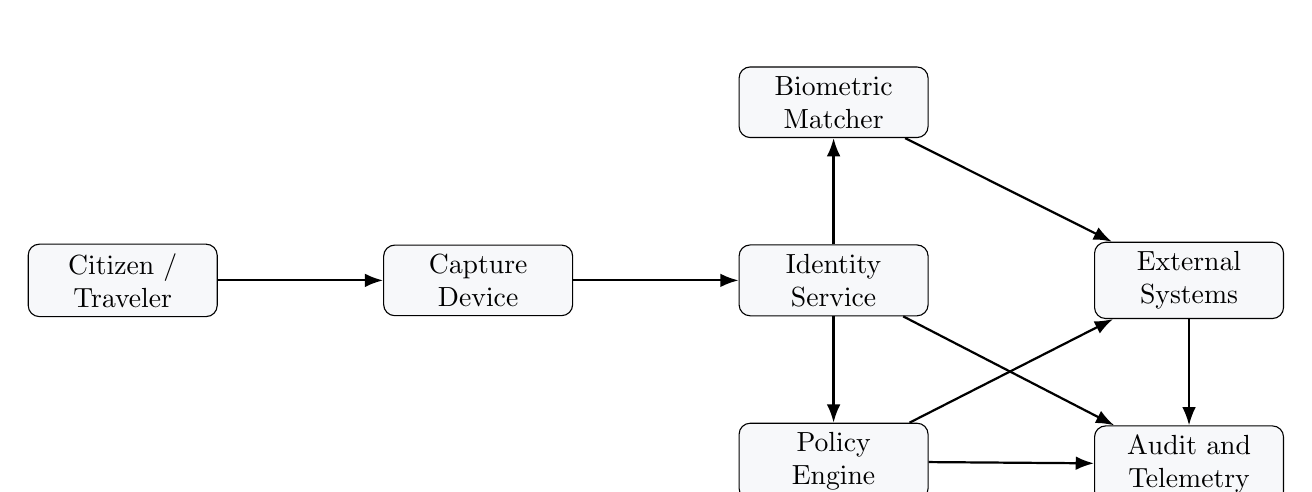
\begin{tikzpicture}[
  node/.style={draw, rounded corners, align=center, minimum width=2.4cm, minimum height=0.8cm, fill=softgray},
  arrow/.style={-Latex, thick}
]
\node[node] (citizen) {Citizen /\\Traveler};
\node[node, right=2.1cm of citizen] (capture) {Capture\\Device};
\node[node, right=2.1cm of capture] (identity) {Identity\\Service};
\node[node, above=1.35cm of identity] (bio) {Biometric\\Matcher};
\node[node, below=1.35cm of identity] (policy) {Policy\\Engine};
\node[node, right=2.1cm of identity] (external) {External\\Systems};
\node[node, below=1.35cm of external] (audit) {Audit and\\Telemetry};

\draw[arrow] (citizen) -- (capture);
\draw[arrow] (capture) -- (identity);
\draw[arrow] (identity) -- (bio);
\draw[arrow] (identity) -- (policy);
\draw[arrow] (policy) -- (external);
\draw[arrow] (bio) -- (external);
\draw[arrow] (identity) -- (audit);
\draw[arrow] (policy) -- (audit);
\draw[arrow] (external) -- (audit);
\end{tikzpicture}
\caption{Complex identity and biometric validation as a system-of-systems problem.}
\end{figure}

% ------------------------------------------------------------
\section{Parametrized Testing and the Truth Matrix}
% ------------------------------------------------------------

Once strategic reasoning is complete, automation becomes powerful. At that point, engineers have defined:
\begin{itemize}
\item hypotheses to validate;
\item assumptions to challenge;
\item lifecycle states to cover;
\item object states and transitions;
\item input variability;
\item expected outputs;
\item expected artifacts;
\item expected telemetry;
\item preconditions;
\item evidence rules.
\end{itemize}

Generative AI can then help expand combinations.

\subsection{Truth Matrix Definition}

A truth matrix is a governed representation of expected operational truth. It is compatible with model-based testing and property-based testing traditions, but extends them with telemetry, evidence records, and operational-risk decisions \cite{utting,claessen,iso29119}.

It maps:
\begin{itemize}
\item scenario context;
\item citizen or object state;
\item identity lifecycle state;
\item biometric condition;
\item input variables;
\item expected decision;
\item expected outputs;
\item expected telemetry;
\item expected artifacts;
\item evidence acceptance criteria.
\end{itemize}

\begin{longtable}{p{2.3cm}p{2.1cm}p{2.2cm}p{2.2cm}p{2.2cm}p{2.8cm}}
\toprule
\textbf{Citizen State} & \textbf{Identity State} & \textbf{Biometric Context} & \textbf{Operational Context} & \textbf{Decision} & \textbf{Expected Evidence} \\
\midrule
New applicant & Not enrolled & Good quality capture & Normal enrollment & Enroll & Enrollment event, identity record, audit trace \\
Active traveler & Active & Good match score & Border crossing & Approve & Verification span, policy span, audit event \\
Watchlisted person & Active & Match score above threshold & High risk context & Escalate & Alert event, supervisor workflow, full trace chain \\
Expired credential & Inactive & Any biometric input & Normal context & Deny & Denial event, lifecycle reason, audit record \\
Presentation attack & Active & Spoof attempt & Remote verification & Reject & PAD alert, rejection decision, evidence package \\
\bottomrule
\end{longtable}

The AI may explore combinations. It may suggest additional rows. It may generate candidate cases. But the meaning of ``true'' remains defined by engineers.

% ------------------------------------------------------------
\section{Telemetry as Oracle}
% ------------------------------------------------------------

In traditional testing, the oracle is often an expected output. In complex operational systems, the oracle must also include telemetry.

\strongclaim{Telemetry is not merely a debugging aid. In evidence-centric testing, telemetry is part of the oracle.}

OpenTelemetry (OTel) is used here as a representative standard for traces, metrics, logs, context propagation, and semantic instrumentation \cite{opentelemetry}. The broader idea is independent of any single tooling stack: observability artifacts can become evidence artifacts.

\subsection{Expected Observability Signals}

A test scenario should specify expected:
\begin{itemize}
\item traces;
\item span names;
\item span IDs and trace IDs;
\item parent-child relationships;
\item business events;
\item logs;
\item metrics;
\item audit artifacts;
\item evidence packages.
\end{itemize}

Example: a biometric verification scenario may require:
\begin{itemize}
\item one capture span;
\item one biometric-quality-evaluation span;
\item one matcher span;
\item one policy-decision span;
\item one audit-write span;
\item consistent trace ID propagation;
\item required attributes such as transaction ID, identity lifecycle state, and decision reason.
\end{itemize}

If the output is correct but the telemetry chain is broken, the evidence is incomplete.

\subsection{Same Trace ID and Evidence Continuity}

A critical requirement is trace continuity. When a test runs, the evidence should be retrievable through trace IDs and span IDs across the lifecycle.

This enables:
\begin{itemize}
\item reconstruction of the execution path;
\item verification of expected business events;
\item isolation of failure causes;
\item automated evidence collection;
\item auditability of test decisions.
\end{itemize}

% ------------------------------------------------------------
\section{AI-Assisted Verification of Governed Controls}
% ------------------------------------------------------------

The paper does not reject generative AI. On the contrary, it argues for a more mature use of it.

AI can help verify controls defined by engineers.

Examples include:
\begin{itemize}
\item checking whether JSON payloads comply with schemas;
\item verifying that generated datasets respect defined constraints;
\item comparing observed traces against expected trace topology;
\item detecting missing spans or missing audit events;
\item checking whether expected artifacts were produced;
\item identifying inconsistencies between requirements, test cases, and telemetry;
\item generating scripts that perform these checks.
\end{itemize}

The difference is fundamental:

\begin{center}
\begin{tabular}{p{5.6cm}p{7.6cm}}
\toprule
\textbf{Weak pattern} & \textbf{Stronger pattern} \\
\midrule
Ask AI to generate tests and trust the output & Ask AI to help build validators for controls defined by engineers \\
Ask AI to invent test data & Ask AI to build auditable data-generation tools \\
Ask AI to define truth & Engineers define truth; AI explores variability around it \\
Ask AI to replace reasoning & Use AI to accelerate governed execution and verification \\
\bottomrule
\end{tabular}
\end{center}

% ------------------------------------------------------------
\section{Generated Generators}
% ------------------------------------------------------------

One of the core contributions of the paper is the concept of generated generators.

Instead of asking generative AI to directly produce test data, engineers ask it to help build:
\begin{itemize}
\item scripts;
\item data generators;
\item lifecycle simulators;
\item telemetry synthesizers;
\item truth-matrix expanders;
\item schema validators;
\item trace validators.
\end{itemize}

These artifacts are governed as part of the test system.

\subsection{Why Generators Matter}

Generators are valuable because they are:
\begin{itemize}
\item inspectable;
\item reviewable;
\item versioned;
\item reproducible;
\item auditable;
\item linked to requirements;
\item linked to architecture decisions;
\item controlled under configuration management.
\end{itemize}

If the system design changes, the impact can be traced across:
\begin{itemize}
\item input generation;
\item expected outputs;
\item expected signals;
\item expected artifacts;
\item telemetry expectations;
\item validation scripts;
\item evidence packages.
\end{itemize}

\subsection{Generator as Test Evidence}

The generator is not only a tool. It is part of the evidence chain.

A generated dataset without generator provenance is weak evidence. A generated dataset produced by a versioned generator, with parameters, seed, schema, and traceability to requirements, is stronger evidence.

\begin{figure}[H]
\centering
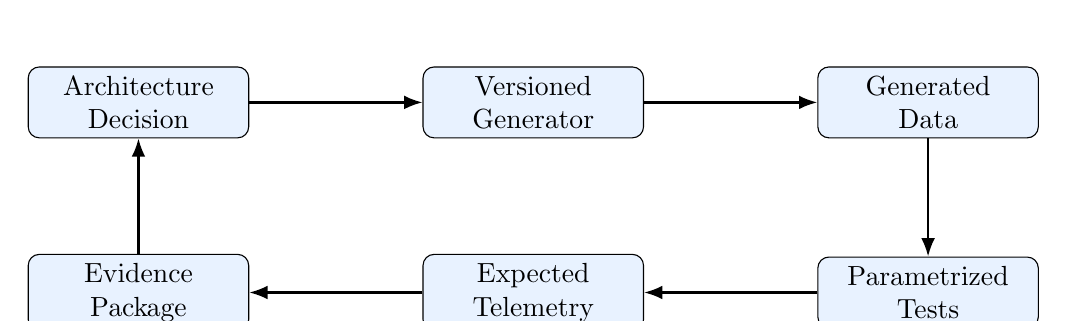
\begin{tikzpicture}[
  node/.style={draw, rounded corners, align=center, minimum width=2.8cm, minimum height=0.85cm, fill=softblue},
  arrow/.style={-Latex, thick}
]
\node[node] (arch) {Architecture\\Decision};
\node[node, right=2.2cm of arch] (generator) {Versioned\\Generator};
\node[node, right=2.2cm of generator] (data) {Generated\\Data};
\node[node, below=1.5cm of data] (tests) {Parametrized\\Tests};
\node[node, left=2.2cm of tests] (telemetry) {Expected\\Telemetry};
\node[node, left=2.2cm of telemetry] (evidence) {Evidence\\Package};

\draw[arrow] (arch) -- (generator);
\draw[arrow] (generator) -- (data);
\draw[arrow] (data) -- (tests);
\draw[arrow] (tests) -- (telemetry);
\draw[arrow] (telemetry) -- (evidence);
\draw[arrow] (evidence) -- (arch);
\end{tikzpicture}
\caption{Generated generators as governed evidence infrastructure.}
\end{figure}

% ------------------------------------------------------------
\section{Practitioner Workflow}
% ------------------------------------------------------------

The model can be implemented as a workflow, and can be aligned with continuous delivery and CI/CD governance practices when evidence gates are treated as part of release readiness \cite{humble}. It does not require every organization to adopt a large methodology at once; it can be introduced progressively.

\begin{enumerate}
\item \textbf{Define the operational claim.} Example: ``remote biometric verification rejects presentation attacks under defined conditions.''
\item \textbf{Document assumptions.} Capture environment, architecture, data, instrumentation, policy, and dependency assumptions.
\item \textbf{Classify hypotheses versus assumptions.} Convert testable assumptions into falsifiable hypotheses where possible.
\item \textbf{Define the truth matrix.} Specify operational states, expected decisions, expected artifacts, and expected telemetry.
\item \textbf{Define evidence rules.} Specify what evidence is required for a pass, fail, inconclusive, or evidence-failure result.
\item \textbf{Build governed generators.} Use human design and AI assistance to produce auditable scripts and data generators.
\item \textbf{Verify preconditions.} Ensure that execution context is coherent before running tests.
\item \textbf{Execute parametrized scenarios.} Generate controlled variability and run tests.
\item \textbf{Validate outputs and telemetry.} Compare decisions, traces, logs, metrics, and artifacts against expectations.
\item \textbf{Produce evidence records.} Store machine-readable evidence packages.
\item \textbf{Update confidence and residual risk.} Interpret evidence against claims and assumptions.
\item \textbf{Decide.} Produce a go, conditional go, no-go, remediation, or risk-acceptance decision.
\end{enumerate}

\begin{figure}[H]
\centering
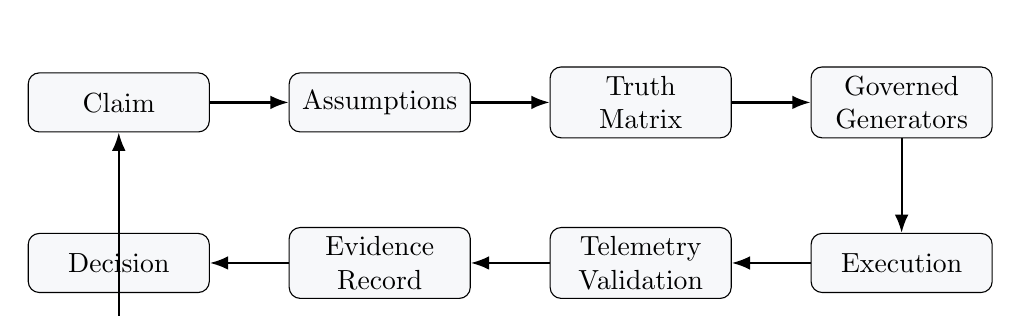
\begin{tikzpicture}[
  wfstep/.style={draw, rounded corners, align=center, minimum width=2.3cm, minimum height=0.75cm, fill=softgray},
  arrow/.style={-Latex, thick}
]
\node[wfstep] (c) {Claim};
\node[wfstep, right=1.0cm of c] (a) {Assumptions};
\node[wfstep, right=1.0cm of a] (t) {Truth\\Matrix};
\node[wfstep, right=1.0cm of t] (g) {Governed\\Generators};

\node[wfstep, below=1.2cm of g] (e) {Execution};
\node[wfstep, left=1.0cm of e] (v) {Telemetry\\Validation};
\node[wfstep, left=1.0cm of v] (r) {Evidence\\Record};
\node[wfstep, left=1.0cm of r] (d) {Decision};

\draw[arrow] (c) -- (a);
\draw[arrow] (a) -- (t);
\draw[arrow] (t) -- (g);
\draw[arrow] (g) -- (e);
\draw[arrow] (e) -- (v);
\draw[arrow] (v) -- (r);
\draw[arrow] (r) -- (d);
\draw[arrow] (d) -- ++(0,-0.8) -| (c);
\end{tikzpicture}
\caption{Implementation workflow for evidence-centric AI-assisted testing. The loop starts with a human-defined operational claim, moves through assumptions, truth matrices, governed generators, execution, telemetry validation, and evidence records, then returns to decision-making through confidence update and residual-risk review.}
\end{figure}

% ------------------------------------------------------------
\section{Preconditions, Inconclusive Results, and Defect Classification}
% ------------------------------------------------------------

A major failure mode in test governance is confusing three categories:
\begin{enumerate}
\item product defect;
\item invalid test context;
\item inconclusive evidence.
\end{enumerate}

A robust test system must differentiate them.

\subsection{Precondition Failure}

If a required precondition is false, the test should not be interpreted as a product failure.

Examples:
\begin{itemize}
\item identity registry unavailable;
\item biometric matcher not synchronized;
\item certificate expired in the environment;
\item test data corrupted;
\item OpenTelemetry collector unavailable;
\item feature flag not aligned with release package.
\end{itemize}

Such cases should trigger environment remediation or test-context correction.

\subsection{Evidence Failure}

If the expected output is correct but evidence is missing, the decision should be cautious. The system may have behaved correctly, but the assurance claim is not fully supported.

This is especially important in regulated systems where auditability is not optional.

% ------------------------------------------------------------
\section{Sociological Dimension: Generative AI and Premature Closure of Ambiguity}
% ------------------------------------------------------------

Testing in complex systems is not only a technical process. It is also a social process of constructing shared understanding.

Test design requires interaction among:
\begin{itemize}
\item architects;
\item product experts;
\item business analysts;
\item QA engineers;
\item operations teams;
\item security experts;
\item legal and compliance stakeholders;
\item customer representatives;
\item domain experts.
\end{itemize}

A test often reveals that the organization itself does not yet agree on what the system is supposed to do.

\subsection{Why Generative AI Changes the Sociology of Testing}

The socio-technical argument is not that AI is the first technology to affect testing work. The argument is that generative AI changes the form of organizational closure. Perrow's analysis of complex and tightly coupled systems warns that small interactions can produce consequences not visible from isolated components \cite{perrow}. Latour's notion of black boxing explains how stabilized technical artifacts can hide the negotiations and assumptions that produced them \cite{latour}. Weick and Sutcliffe's work on high-reliability organizations emphasizes preoccupation with failure, reluctance to simplify, sensitivity to operations, resilience, and deference to expertise \cite{weick}. These concepts matter because test artifacts are not neutral; they shape what an organization believes it knows.

Classic automation executes predefined instructions. Generative AI does something different: it produces fluent artifacts.

It can generate:
\begin{itemize}
\item test plans;
\item acceptance criteria;
\item risk analyses;
\item requirements summaries;
\item test scenarios;
\item evidence reports;
\item executive summaries.
\end{itemize}

This creates a specific sociological risk: premature closure of ambiguity.

\riskbox{
Generative AI may convert unresolved organizational ambiguity into polished apparent certainty.
}

A team may still not agree on:
\begin{itemize}
\item what the system should do;
\item what evidence is sufficient;
\item which assumption is fragile;
\item which lifecycle state matters;
\item what ``valid identity verification'' means operationally.
\end{itemize}

Yet the AI can produce a coherent-looking test plan.

This is more than a technical hallucination problem. It is an organizational knowledge problem. A well-formatted artifact may prematurely close a debate that should remain open until assumptions are clarified. In Latourian terms, unresolved reasoning can become black-boxed too early; in high-reliability terms, the organization may lose its reluctance to simplify \cite{latour,weick}.

\subsection{Quality of Assumptions}

The quality of assumptions can be assessed through:
\begin{itemize}
\item explicit ownership;
\item review date;
\item evidence availability;
\item falsifiability;
\item dependency criticality;
\item impact if false;
\item conversion potential into hypotheses.
\end{itemize}

Weak assumptions are often hidden assumptions. The first governance benefit of this model is making them visible.

\subsection{Preventing Governance Theater}

Evidence-centric testing can be gamed if teams define weak assumptions to make results look better. Countermeasures include:
\begin{itemize}
\item independent assumption review;
\item architecture peer review;
\item traceability to operational incidents;
\item challenge sessions with product and operations experts;
\item explicit residual-risk ownership;
\item evidence completeness metrics.
\end{itemize}

More concrete controls can be introduced progressively:
\begin{itemize}
\item \textbf{Assumption review boards:} lightweight peer reviews for assumptions, similar to code reviews, especially for release-critical claims.
\item \textbf{Assumption red teaming:} assign a reviewer to falsify or stress-test the assumptions behind a truth matrix.
\item \textbf{Incident-linked assumptions:} if an assumption was false in a past incident, outage, audit issue, or defect escape, it must be explicitly revalidated.
\item \textbf{Automated weak-assumption detection:} flag tests that continue to pass even when critical assumptions are perturbed or removed.
\item \textbf{Evidence-threshold gates:} prevent teams from reporting full pass when evidence completeness is below the agreed threshold.
\end{itemize}

The goal is to avoid turning evidence governance into compliance theater. The framework is valuable only if assumptions remain challengeable and evidence remains inspectable.

% ------------------------------------------------------------
\section{Novelty Relative to Existing Testing Traditions}
% ------------------------------------------------------------

This paper does not reject existing testing traditions. It builds on them.

\subsection{Context-Driven Testing}

Context-driven testing established that skilled human judgment, context, investigation, exploratory learning, and testing psychology are central to testing \cite{kaner,bach,myers}. This paper strongly aligns with that tradition.

The novelty is not the claim that humans matter. The novelty is the extension of that principle into AI-assisted, observability-rich, system-of-systems environments.

\begin{longtable}{p{5.2cm}p{8.4cm}}
\toprule
\textbf{Context-Driven Testing} & \textbf{This Paper Adds} \\
\midrule
Human judgment matters & Human-defined truth under AI-assisted generation \\
Context determines strategy & Operational context becomes a first-class validation object \\
Testing is investigation & Testing becomes evidence governance \\
Oracles matter & Telemetry becomes part of the oracle \\
Testers reason under uncertainty & Priors, assumptions, confidence updates, and residual risk are made explicit \\
Tools support testers & AI builds governed generators and validators rather than replacing test reasoning \\
\bottomrule
\end{longtable}

\subsection{Model-Based Testing}

Model-based testing uses models to derive tests from expected system behavior \cite{utting}. Truth matrices and lifecycle-state reasoning resemble this tradition. The contribution here is not to replace model-based testing, but to connect it with:
\begin{itemize}
\item telemetry-as-oracle;
\item generated generators;
\item evidence records;
\item confidence updates;
\item operational-risk decisions.
\end{itemize}

\subsection{Property-Based Testing}

Property-based testing generates inputs to check invariant properties \cite{claessen}. The generated-generator concept is compatible with this approach. The extension proposed here is to apply similar generative discipline to socio-technical operational claims, not only software properties.

\subsection{Chaos Engineering}

Chaos engineering introduces controlled disturbances to test resilience under failure conditions \cite{basiri}. The present model aligns with its emphasis on operational assumptions and steady-state hypotheses. It extends the idea by requiring that the evidence chain itself be validated: not only did the system resist the disturbance, but did we produce the evidence required to trust that conclusion? This is consistent with safety engineering and high-reliability thinking, where awareness of weak signals and operational sensitivity matter as much as formal success \cite{hollnagel,weick}.

% ------------------------------------------------------------
\section{Case Studies}
% ------------------------------------------------------------

\subsection{Case Study 1: Biometric Verification With Broken Audit Chain}

\textbf{Scenario.} A remote biometric verification workflow rejects a presentation attack. The functional output is correct.

\textbf{Traditional result.} Test passed.

\textbf{Evidence-centric result.} Conditional failure.

\textbf{Reason.} The expected PAD alert was produced, but the audit-write span was missing and the trace chain could not reconstruct the end-to-end decision path.

\textbf{Conclusion.} The product behavior may be correct, but operational assurance is incomplete.

\subsection{Case Study 2: Border-Control Workflow With Stale Watchlist}

\textbf{Scenario.} A traveler is processed through a border-control identity verification workflow. The verification output is \texttt{APPROVE}.

\textbf{Traditional result.} Test passed if the expected output was approve.

\textbf{Evidence-centric result.} Inconclusive or invalid test context.

\textbf{Reason.} Precondition checks reveal that the watchlist synchronization timestamp is outside the acceptable freshness threshold.

\textbf{Conclusion.} The system decision cannot be interpreted without validating the operational context.

\subsection{Case Study 3: Identity Lifecycle Drift Across Systems}

\textbf{Scenario.} A credential is marked expired in the civil registry but remains active in a downstream verification service.

\textbf{Traditional result.} Individual service tests may pass locally.

\textbf{Evidence-centric result.} System-of-systems inconsistency.

\textbf{Reason.} The truth matrix expects lifecycle-state consistency across registry, policy engine, verification service, and audit system.

\textbf{Conclusion.} The defect is not localized assertion failure. It is an operational truth propagation failure.

% ------------------------------------------------------------
\section{AI-Assisted Doubt Under Human Governance}
% ------------------------------------------------------------

The paper should not be read as anti-AI. A more precise position is that AI can assist doubt, but should not own the final definition of truth.

Under human governance, AI can be used as:
\begin{itemize}
\item \textbf{a devil's advocate:} challenge a truth matrix by proposing edge cases, missing lifecycle states, or inconsistent assumptions;
\item \textbf{an assumption gap detector:} scan requirements, architecture notes, test cases, and telemetry rules to identify assumptions that were never written down;
\item \textbf{a scenario stressor:} propose degraded-mode, adversarial, latency, synchronization, or configuration-drift situations;
\item \textbf{a trace reviewer:} compare expected trace topology against observed trace topology and flag missing spans or broken context propagation;
\item \textbf{a consistency checker:} detect contradictions between expected outputs, lifecycle states, and evidence rules.
\end{itemize}

The governance boundary is essential. AI may propose doubts. Humans must decide which doubts matter, which assumptions become governed, which hypotheses require testing, and which residual risks can be accepted.

% ------------------------------------------------------------
\section{Tooling and Implementation Mapping}
% ------------------------------------------------------------

This whitepaper is intentionally tool-agnostic, but practical implementation can reuse existing platforms.

\begin{longtable}{p{4cm}p{9.5cm}}
\toprule
\textbf{Need} & \textbf{Possible Tooling Direction} \\
\midrule
Truth matrix & CSV/YAML matrices, Cucumber scenario outlines, Gherkin tables, XRAY, Polarion, Jira, custom governance repositories \\
Parametrized generation & Python, property-based testing tools, Hypothesis, custom generators, model-based test generation \\
Generator governance & Git, pull requests, code review, semantic versioning, configuration management \\
Telemetry oracle & OpenTelemetry SDKs, collectors, Jaeger, Tempo, Prometheus, Loki, Elastic, custom span-topology validators \\
Evidence record & JSON evidence packages, Allure reports, XRAY evidence attachments, immutable artifact stores \\
Trace validation & Span-topology rules, trace ID continuity checks, expected event validation, schema-based telemetry verification \\
Risk dashboard & Grafana, custom BI dashboards, Jira/XRAY reports, STRAT-Q decision boards \\
Precondition verification & Shell/Python scripts, health checks, contract checks, environment drift detectors \\
\bottomrule
\end{longtable}

The key point is not the tool itself. The key point is that test data, telemetry, evidence, and decisions must be connected through a governed chain.

\subsection{Example End-to-End Tool Integration}

A practical implementation could combine existing tools:
\begin{itemize}
\item define the truth matrix in YAML and expose selected scenarios as Cucumber/Gherkin scenario outlines;
\item build parametrized generators in Python, optionally using property-based testing libraries for controlled variability;
\item version generator code, truth matrices, and evidence rules in Git;
\item instrument the system using OpenTelemetry SDKs and collect traces through an OpenTelemetry Collector;
\item validate trace topology through a custom span validator that checks required spans, attributes, parent-child relationships, and trace continuity;
\item store evidence packages in Allure, XRAY attachments, or an immutable artifact repository;
\item enforce CI/CD gates in Jenkins, GitHub Actions, or equivalent tooling when evidence completeness falls below threshold.
\end{itemize}

This is deliberately incremental. Organizations do not need a new platform to begin. They need to connect existing quality, telemetry, and configuration-management practices into a single evidence chain.

% ------------------------------------------------------------
\section{Evaluation Metrics}
% ------------------------------------------------------------

The effectiveness of an evidence-centric AI-assisted testing approach should not be measured only by number of tests generated.

Recommended metrics include:
\begin{itemize}
\item percentage of tests linked to explicit claims;
\item percentage of tests with documented assumptions;
\item percentage of assumptions with owners and review dates;
\item percentage of assumptions converted into falsifiable hypotheses;
\item percentage of scenarios with truth-matrix coverage;
\item precondition verification success rate;
\item evidence completeness score;
\item trace continuity rate;
\item telemetry-oracle conformance rate;
\item percentage of tests with retrievable logs, traces, metrics, and artifacts;
\item number of architecture ambiguities discovered during test design;
\item number of operational-context failures detected before execution;
\item residual-risk reduction per test effort unit.
\end{itemize}

\subsection{Evidence Completeness Score}

An evidence completeness score can be defined as:

\[
ECS = \frac{ObservedRequiredEvidence}{ExpectedRequiredEvidence}
\]

where expected required evidence includes:
\begin{itemize}
\item output result;
\item trace chain;
\item required spans;
\item required business events;
\item logs;
\item metrics;
\item audit artifacts;
\item generator provenance;
\item environment precondition record.
\end{itemize}

For high-assurance systems, a passed assertion with low evidence completeness should not be considered a full pass.

% ------------------------------------------------------------
\section{Minimal Evidence Record}
% ------------------------------------------------------------

Each test execution should produce an evidence record similar to:

\begin{lstlisting}
{
  "test_id": "BIO-VERIFY-ATTACK-042",
  "claim": "Presentation attacks are rejected under remote verification conditions",
  "assumptions": [
    {
      "id": "A-001",
      "statement": "PAD service is enabled",
      "owner": "Security QA",
      "review_date": "2026-06-01"
    },
    {
      "id": "A-002",
      "statement": "OTel collector is reachable",
      "owner": "DevOps",
      "review_date": "2026-06-01"
    }
  ],
  "prior": {
    "claim_valid_probability": 0.70,
    "prior_model": "Beta(7,3)",
    "source": ["architecture_review", "previous_incidents", "expert_elicitation"],
    "confidence_in_prior": "medium"
  },
  "input_generator": {
    "name": "biometric_variability_generator",
    "version": "1.4.2",
    "seed": "20260515-042",
    "repository_commit": "a17f92c"
  },
  "expected_decision": "REJECT",
  "expected_events": ["PAD_ALERT", "AUDIT_REJECTION"],
  "expected_trace_topology": [
    "capture",
    "quality_check",
    "pad_detection",
    "policy_decision",
    "audit_write"
  ],
  "actual_decision": "REJECT",
  "trace_id": "abc123",
  "evidence_status": "COMPLETE",
  "evidence_completeness_score": 1.0,
  "confidence_update": "positive",
  "residual_risk": "reduced but not eliminated",
  "decision": "conditional_go_pending_edge_case_review"
}
\end{lstlisting}

% ------------------------------------------------------------
\section{Counterarguments and Scope Boundaries}
% ------------------------------------------------------------

\subsection{Objection 1: This Sounds Expensive}

Yes. Evidence-centric governance has a cost.

The response is proportionality. Risk-management frameworks similarly emphasize tailoring governance to the context, impact, and use case \cite{nistai,nistgenai}. Not every system needs this level of rigor. However, in systems where identity, public trust, legal responsibility, safety, border operations, elections, or national-scale services are involved, the cost of insufficient evidence may exceed the cost of governance.

\subsection{Objection 2: Not All Systems Need This}

Correct.

This model should be scaled according to criticality:
\begin{itemize}
\item lightweight for low-risk digital services;
\item moderate for business-critical platforms;
\item rigorous for regulated identity, biometric, border, election, and mission-critical systems.
\end{itemize}

The purpose is not bureaucracy. The purpose is proportional assurance.

\subsection{Objection 3: AI Can Help With Doubt}

Yes, but with boundaries.

AI can surface edge cases, contradictions, missing scenarios, weak assumptions, and gaps in the truth matrix. However, humans remain accountable for defining evidence boundaries, accepting residual risk, and making operational decisions.

\subsection{Objection 4: This Is Just Better Documentation}

No.

Documentation records what was intended. Evidence-centric testing connects intention, execution, telemetry, generated data, and decision. It is not merely documentation; it is a governed evidence-production system.

% ------------------------------------------------------------
\section{Engineering Governance Model}
% ------------------------------------------------------------

We propose an engineering governance model with two planes:
\begin{itemize}
\item a \textbf{reasoning plane}, where humans define claims, assumptions, hypotheses, truth matrices, and evidence rules;
\item an \textbf{industrialization plane}, where AI, scripts, and automation expand variability and verify governed controls.
\end{itemize}

\begin{figure}[H]
\centering
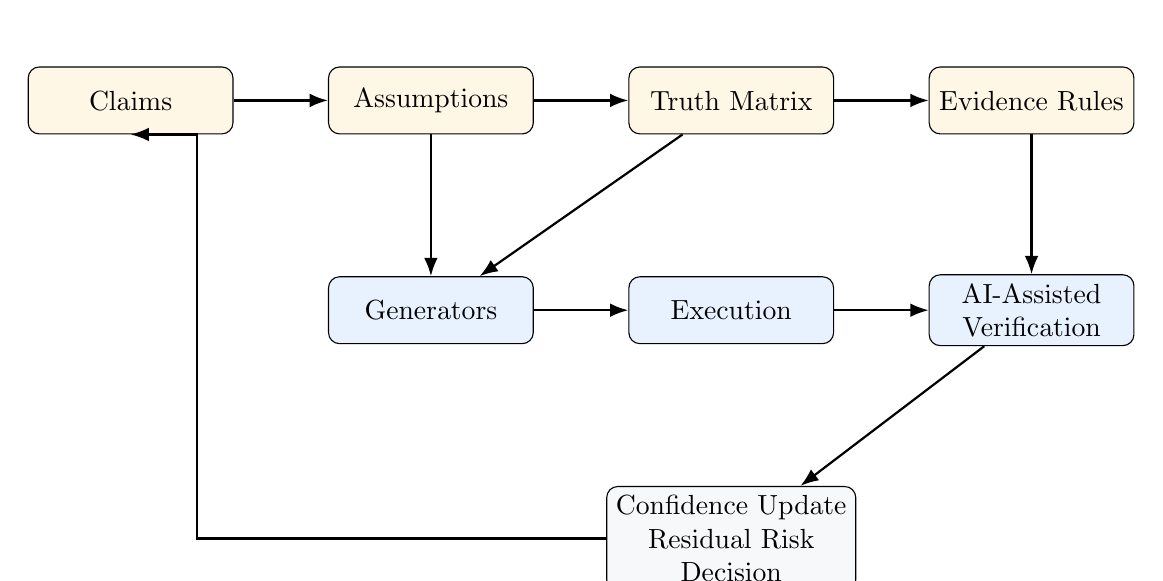
\begin{tikzpicture}[
  box/.style={draw, rounded corners, align=center, minimum width=2.6cm, minimum height=0.85cm},
  hbox/.style={box, fill=softamber},
  abox/.style={box, fill=softblue},
  arrow/.style={-Latex, thick}
]
\node[hbox] (claim) {Claims};
\node[hbox, right=1.2cm of claim] (assump) {Assumptions};
\node[hbox, right=1.2cm of assump] (truth) {Truth Matrix};
\node[hbox, right=1.2cm of truth] (evidence) {Evidence Rules};

\node[abox, below=1.8cm of assump] (gen) {Generators};
\node[abox, right=1.2cm of gen] (exec) {Execution};
\node[abox, right=1.2cm of exec] (verify) {AI-Assisted\\Verification};

\node[box, fill=softgray, below=1.8cm of exec] (decision) {Confidence Update\\Residual Risk\\Decision};

\draw[arrow] (claim) -- (assump);
\draw[arrow] (assump) -- (truth);
\draw[arrow] (truth) -- (evidence);
\draw[arrow] (evidence) -- (verify);
\draw[arrow] (assump) -- (gen);
\draw[arrow] (truth) -- (gen);
\draw[arrow] (gen) -- (exec);
\draw[arrow] (exec) -- (verify);
\draw[arrow] (verify) -- (decision);
\draw[arrow] (decision.west) -- ++(-5.2,0) |- (claim.south);
\end{tikzpicture}
\caption{Human-defined reasoning plane and AI-assisted industrialization plane.}
\end{figure}

% ------------------------------------------------------------
\section{Implications for QA Leadership and Engineering Management}
% ------------------------------------------------------------

The proposed approach changes the role of QA leadership.

The QA leader is no longer only responsible for:
\begin{itemize}
\item test execution;
\item defect detection;
\item automation coverage;
\item reporting.
\end{itemize}

The QA leader becomes responsible for:
\begin{itemize}
\item evidence governance;
\item operational risk compression;
\item traceability from requirement to evidence;
\item quality of assumptions;
\item confidence-aware decision support;
\item cross-functional alignment around truth.
\end{itemize}

This is especially important in organizations where testing is often perceived as late-stage verification. In complex systems, testing should begin as early operational reasoning.

% ------------------------------------------------------------
\section{Limitations}
% ------------------------------------------------------------

This paper is a conceptual and architectural whitepaper. It does not claim that the proposed model is universally applicable without adaptation.

Limitations include:
\begin{itemize}
\item evidence-centric testing requires mature observability;
\item truth matrices require domain expertise and governance effort;
\item generated generators require configuration management discipline;
\item telemetry validation may produce noise if instrumentation is unstable;
\item sociological adoption may be harder than technical implementation;
\item not all systems require this level of assurance.
\end{itemize}

However, for mission-critical identity, biometric, border, election, and public-service ecosystems, these costs may be justified by the operational and reputational risk profile.

% ------------------------------------------------------------
\section{Future Work}
% ------------------------------------------------------------

Future work should be prioritized according to feasibility, impact, and adoption cost.

\begin{longtable}{p{5.2cm}p{2.2cm}p{2.0cm}p{2.0cm}p{2.0cm}}
\toprule
\textbf{Future Work Item} & \textbf{Feasibility} & \textbf{Impact} & \textbf{Priority} & \textbf{Rationale} \\
\midrule
CI/CD gates based on evidence completeness & High & High & P0 & Directly actionable with existing pipelines and telemetry stores \\
Trace-topology validators for OpenTelemetry evidence & High & High & P0 & Turns observability into executable evidence rules \\
Truth matrix integration with model-based testing and architecture descriptions \cite{iso42010,utting} & High & Medium & P1 & Connects test design with system models and architecture rationale \\
Bayesian networks for residual-risk propagation & Medium & High & P1 & Useful for critical systems where assumptions and claims are dependent \\
STRAT-Q-style residual-risk dashboards & Medium & Medium & P2 & Helps executives see evidence, confidence, and residual risk together \\
Cross-functional truth reviews or evidence councils & Low/Medium & High & P2 & High governance value but culturally harder to adopt \\
Application to PAD, identity lifecycle transitions, and border-control workflows & Medium & High & P1 & Strong domain relevance for biometric and identity ecosystems \\
\bottomrule
\end{longtable}

This roadmap intentionally starts with practical evidence gates and trace validation because they are easier to pilot and demonstrate quickly.

% ------------------------------------------------------------
\section{Conclusion}
% ------------------------------------------------------------

Generative AI can help produce tests. More importantly, it can help industrialize variability after engineers have defined the operational model.

But the strategic value of testing does not reside in mechanical production. It resides in doubt, priors, assumptions, hypotheses, architecture challenge, context validation, evidence design, and risk-informed decision-making.

AI can help build generators. AI can help verify governed controls. AI can help compare telemetry against expected patterns. AI can help scale parametrized exploration.

But engineers remain responsible for defining truth.

\begin{center}
\Large
\textbf{AI can generate plausibility.}\\[0.2cm]
\textbf{Engineers remain accountable for operational truth.}\\[0.4cm]
\textbf{The future of testing is not automated plausibility.}\\[0.2cm]
\textbf{It is governed evidence.}
\end{center}

\newpage

% ------------------------------------------------------------
\begin{thebibliography}{99}

\bibitem{nist80063}
National Institute of Standards and Technology.
\textit{Digital Identity Guidelines, NIST Special Publication 800-63 Revision 4}.
NIST, 2025. Available at: \url{https://pages.nist.gov/800-63-4/}

\bibitem{nistai}
National Institute of Standards and Technology.
\textit{Artificial Intelligence Risk Management Framework (AI RMF 1.0)}.
NIST, 2023. Available at: \url{https://www.nist.gov/itl/ai-risk-management-framework}

\bibitem{nistgenai}
National Institute of Standards and Technology.
\textit{Artificial Intelligence Risk Management Framework: Generative Artificial Intelligence Profile, NIST AI 600-1}.
NIST, 2024. DOI: \url{https://doi.org/10.6028/NIST.AI.600-1}.

\bibitem{opentelemetry}
OpenTelemetry Project.
\textit{OpenTelemetry Documentation and Specification}.
Cloud Native Computing Foundation. Available at: \url{https://opentelemetry.io/docs/}

\bibitem{iso30107}
ISO/IEC.
\textit{ISO/IEC 30107-1:2016, Information technology - Biometric presentation attack detection - Part 1: Framework}.
International Organization for Standardization, 2016. Available at: \url{https://www.iso.org/standard/53227.html}.

\bibitem{iso301073}
ISO/IEC.
\textit{ISO/IEC 30107-3:2017, Information technology - Biometric presentation attack detection - Part 3: Testing and reporting}.
International Organization for Standardization, 2017. Available at: \url{https://www.iso.org/standard/67381.html}.

\bibitem{iso29119}
ISO/IEC/IEEE.
\textit{ISO/IEC/IEEE 29119 Software and systems engineering - Software testing}.
International Organization for Standardization / International Electrotechnical Commission / IEEE. See for example: \url{https://www.iso.org/standard/81291.html}.

\bibitem{iso42010}
ISO/IEC/IEEE.
\textit{ISO/IEC/IEEE 42010:2022, Software, systems and enterprise - Architecture description}.
International Organization for Standardization / International Electrotechnical Commission / IEEE. Available at: \url{https://www.iso.org/standard/74393.html}.

\bibitem{etsi119461}
ETSI.
\textit{ETSI TS 119 461 v2.1.1 (February 2025), Electronic Signatures and Trust Infrastructures (ESI) - Policy and security requirements for trust service components providing identity proofing of trust service subjects}.
European Telecommunications Standards Institute, 2025. Available at: \url{https://www.etsi.org/deliver/etsi_ts/119400_119499/119461/02.01.01_60/ts_119461v020101p.pdf}

\bibitem{cnilbio}
CNIL.
\textit{Biometrie: definitions et enjeux}.
Commission Nationale de l'Informatique et des Libertes. Available at: \url{https://www.cnil.fr/fr/biometrie}

\bibitem{nistbio}
National Institute of Standards and Technology.
\textit{Biometrics and Biometric Technology Evaluations}.
NIST. Available at: \url{https://www.nist.gov/programs-projects/biometrics}

\bibitem{goodenough}
Goodenough, J. B., and Gerhart, S. L.
\textit{Toward a theory of test data selection}.
IEEE Transactions on Software Engineering, 1975. DOI: \url{https://doi.org/10.1109/TSE.1975.6312836}.

\bibitem{myers}
Myers, G. J., Sandler, C., and Badgett, T.
\textit{The Art of Software Testing}.
Wiley, third edition, 2011. Available at: \url{https://www.wiley.com/en-us/The+Art+of+Software+Testing%2C+3rd+Edition-p-9781118031964}.

\bibitem{kaner}
Kaner, C., Bach, J., and Pettichord, B.
\textit{Lessons Learned in Software Testing: A Context-Driven Approach}.
Wiley, 2001. Available at: \url{https://www.wiley.com/en-us/Lessons+Learned+in+Software+Testing%3A+A+Context+Driven+Approach-p-9780471081128}.

\bibitem{bach}
Bach, J.
\textit{Exploratory Testing Explained}.
Satisfice, 2003. Available at: \url{http://www.satisfice.com/articles/et-article.pdf}.

\bibitem{perrow}
Perrow, C.
\textit{Normal Accidents: Living with High-Risk Technologies}.
Princeton University Press, 1999. Available at: \url{https://press.princeton.edu/books/paperback/9780691004129/normal-accidents}.

\bibitem{latour}
Latour, B.
\textit{Science in Action: How to Follow Scientists and Engineers Through Society}.
Harvard University Press, 1987. Available at: \url{https://www.hup.harvard.edu/books/9780674792913}.

\bibitem{weick}
Weick, K. E., and Sutcliffe, K. M.
\textit{Managing the Unexpected: Sustained Performance in a Complex World}.
Jossey-Bass, 2015. Available at: \url{https://www.wiley.com/en-us/Managing+the+Unexpected%3A+Sustained+Performance+in+a+Complex+World%2C+3rd+Edition-p-9781118862414}.

\bibitem{gawande}
Gawande, A.
\textit{The Checklist Manifesto: How to Get Things Right}.
Metropolitan Books, 2009. Available at: \url{https://us.macmillan.com/books/9780312430009/thechecklistmanifesto}.

\bibitem{hollnagel}
Hollnagel, E.
\textit{Safety-I and Safety-II: The Past and Future of Safety Management}.
Ashgate, 2014. Bibliographic reference: \url{https://portal.findresearcher.sdu.dk/en/publications/safety-i-and-safety-ii-the-past-and-future-of-safety-management}.

\bibitem{humble}
Humble, J., and Farley, D.
\textit{Continuous Delivery: Reliable Software Releases through Build, Test, and Deployment Automation}.
Addison-Wesley, 2010. Available at: \url{https://continuousdelivery.com/book/}.

\bibitem{basiri}
Basiri, A., Behnam, N., de Rooij, R., Hochstein, L., Kosewski, L., Reynolds, J., and Rosenthal, C.
\textit{Chaos Engineering}.
IEEE Software, 2016. DOI: \url{https://doi.org/10.1109/MS.2016.60}.

\bibitem{claessen}
Claessen, K., and Hughes, J.
\textit{QuickCheck: A Lightweight Tool for Random Testing of Haskell Programs}.
ACM SIGPLAN Notices, 2000. DOI: \url{https://doi.org/10.1145/351240.351266}.

\bibitem{utting}
Utting, M., Pretschner, A., and Legeard, B.
\textit{A taxonomy of model-based testing approaches}.
Software Testing, Verification and Reliability, 2012. DOI: \url{https://doi.org/10.1002/stvr.456}.

\bibitem{barrett}
Barrett, A. M., Hendrycks, D., Newman, J., and Nonnecke, B.
\textit{Actionable Guidance for High-Consequence AI Risk Management}.
arXiv:2206.08966, 2022. Available at: \url{https://arxiv.org/abs/2206.08966}.

\bibitem{madhavan}
Madhavan, K., Yazdinejad, A., Zarrinkalam, F., and Dehghantanha, A.
\textit{Quantifying Security Vulnerabilities: A Metric-Driven Security Analysis of Gaps in Current AI Standards}.
arXiv:2502.08610, 2025. Available at: \url{https://arxiv.org/abs/2502.08610}.

\end{thebibliography}

\appendix

% ------------------------------------------------------------
\section{Appendix A: Example Generator Specification}
% ------------------------------------------------------------

\begin{lstlisting}
generator:
  name: biometric_variability_generator
  version: 1.4.2
  seed_policy: deterministic_per_test_id

parameters:
  citizen_state:
    - new_applicant
    - active_traveler
    - watchlisted
    - expired_document

  biometric_context:
    - good_quality_capture
    - low_light
    - partial_face
    - presentation_attack

  operational_context:
    - normal
    - degraded_network
    - border_congestion
    - registry_latency

expected_artifacts:
  - generated_input_payload
  - expected_decision
  - expected_trace_topology
  - expected_audit_event
  - evidence_record
\end{lstlisting}

% ------------------------------------------------------------
\section{Appendix B: Example Trace Validation Rule}
% ------------------------------------------------------------

\begin{lstlisting}
rule: biometric_verification_trace_complete

required_spans:
  - capture
  - quality_check
  - biometric_match
  - policy_decision
  - audit_write

required_attributes:
  - transaction_id
  - identity_state
  - biometric_score
  - decision_reason

validation:
  same_trace_id: true
  missing_span_behavior: fail_evidence
  wrong_decision_behavior: fail_product
\end{lstlisting}

% ------------------------------------------------------------
\section{Appendix C: Example Assumption Register}
% ------------------------------------------------------------

\begin{longtable}{p{3cm}p{4cm}p{3cm}p{3cm}}
\toprule
\textbf{Assumption} & \textbf{Risk if False} & \textbf{Owner} & \textbf{Review Trigger} \\
\midrule
Matcher threshold is aligned with policy & False accept or false reject decision & Architecture / Product & Policy change \\
Presentation Attack Detection service is active & Spoofing scenario not valid & Security / QA & Release deployment \\
OpenTelemetry collector reachable & Evidence incomplete & DevOps / QA & Environment change \\
Test data representative & False confidence & QA / Product & Dataset update \\
Watchlist freshness within threshold & Wrong border decision & Operations / Security & Synchronization delay \\
\bottomrule
\end{longtable}

% ------------------------------------------------------------
\section{Appendix D: Acronyms}
% ------------------------------------------------------------

\begin{longtable}{p{3cm}p{10cm}}
\toprule
\textbf{Acronym} & \textbf{Meaning} \\
\midrule
AI & Artificial Intelligence \\
CI/CD & Continuous Integration / Continuous Delivery or Deployment \\
ECS & Evidence Completeness Score \\
LLM & Large Language Model \\
MBT & Model-Based Testing \\
OTel & OpenTelemetry \\
PAD & Presentation Attack Detection \\
QA & Quality Assurance \\
STRAT-Q & Strategic Quality / risk-compression framing used as a conceptual foundation in this work \\
\bottomrule
\end{longtable}

\end{document}
